
\PassOptionsToPackage{table,xcdraw}{xcolor}
% * <majingyisunshine@gmail.com> 2018-05-19T11:43:51.775Z:
%
% ^.
\documentclass[
	dbse, 		 % include logo of DBSE working group
  %draft,    % omit title page, listings, and particular chapters selected below using include only
	%german,   % titles for a thesis in German, A4 paper
	print,    % the printed version does not use colored links
	final,    % removes all TODOs
]{tex/ttthesis}
 
% Color Scheme http://colorschemedesigner.com/#3w40I--ALK-K-
% Base Color of the OVGU INF logo, tetraed, -45
\definecolor{blue1}{RGB}{0,105,180} % gray 95
\definecolor{blue2}{RGB}{40,87,121}
\definecolor{blue3}{RGB}{0,57,97}
\definecolor{blue4}{RGB}{76,166,230}
\definecolor{blue5}{RGB}{136,191,230}
\definecolor{orange1}{RGB}{255,144,0} % gray 133
\definecolor{orange2}{RGB}{171,121,56}
\definecolor{orange3}{RGB}{137,78,0}
\definecolor{orange4}{RGB}{255,181,84}
\definecolor{orange5}{RGB}{255,210,151}
\definecolor{green1}{RGB}{11,215,0} % gray 75
\definecolor{green2}{RGB}{52,144,48}
\definecolor{green3}{RGB}{6,116,0}
\definecolor{green4}{RGB}{88,241,80}
\definecolor{green5}{RGB}{148,241,143}
\definecolor{red1}{RGB}{253,0,6} % gray 86
\definecolor{red2}{RGB}{170,56,59}
\definecolor{red3}{RGB}{136,0,3}
\definecolor{red4}{RGB}{254,84,88}
\definecolor{red5}{RGB}{254,151,154}

\definecolor{background}{named}{white}
\definecolor{bgborder}{named}{black}
\definecolor{comment}{named}{red3}

\definecolor{blue}{named}{blue1}
\definecolor{green}{named}{green1}
\definecolor{red}{named}{red1}
\definecolor{orange}{named}{orange1}

\definecolor{pdflinkcolor}{named}{blue3}
\definecolor{pdfcitecolor}{named}{green3}

\usepackage{listings} % source code listings

%\renewcommand\lstlistingname{Quelltext}

\lstdefinestyle{java}{
%code formatting
	language=Java,
	tabsize=4,
	breaklines=false,
	basicstyle=\fontfamily{pcr}\footnotesize\selectfont,
	commentstyle=\fontshape{it}\color{darkgray}\selectfont,
	keywordstyle=\fontseries{b}\selectfont,
	stringstyle=\fontfamily{cmr}\selectfont,
%line numbering
	numbers=left,
	numberstyle=\footnotesize,
%frame properties
	captionpos=b,
	frame=single,%trblTRBL
	framesep=3pt,
	xleftmargin=4pt,
	xrightmargin=4pt,
	rulecolor=\color{bgborder},
}

\usepackage{pgfplots}
\usepackage{tikz}
	\usetikzlibrary{arrows,positioning,backgrounds,fit,trees} 
	\usetikzlibrary{fadings,shapes.geometric}
	\usetikzlibrary{decorations,scopes,calc,decorations.pathreplacing}

\ifgerman{
	\pgfplotsset{tick label style={/pgf/number format/1000 sep=.,/pgf/number format/use comma}}
}

% Tortendiagramme
\newcommand{\slice}[4]{
  \pgfmathparse{0.5*#1+0.5*#2}
  \let\midangle\pgfmathresult

  % slice
  \draw[thick,
	%fill=background
	] (0,0) -- (#1:1) arc (#1:#2:1) -- cycle;

  % outer label
  \node[label=\midangle:#4] at (\midangle:1) {};

  % inner label
  \pgfmathparse{min((#2-#1-10)/110*(-0.3),0)}
  \let\temp\pgfmathresult
  \pgfmathparse{max(\temp,-0.5) + 0.8}
  \let\innerpos\pgfmathresult
  \node at (\midangle:\innerpos) {#3};
}
\newcommand{\mypiechart}[2]{
	\begin{tikzpicture}[scale=#1]
		\newcounter{a}
		\newcounter{b}
		\foreach \p/\t in {#2}
			{
				\setcounter{a}{\value{b}}
				\addtocounter{b}{\p}
				\slice{\thea/100*360}
							{\theb/100*360}
							{\p\%}{\t}
			}
	\end{tikzpicture}
}

% surrounding TODOs with this command, gives you the ability to remove all if necessary
\iffinal{
	\newcommand{\todo}[1]{}
	\newcommand{\todots}{}
}{
	\newcommand{\todo}[1]{{\color{comment}\textit{[#1]}}}
	\newcommand{\todots}{\todo{\ldots}}
}

% propositional formulas
\newcommand{\pand}{\wedge}
\newcommand{\por}{\vee}
\newcommand{\pnot}{\neg}
\newcommand{\pequals}{\Leftrightarrow}
\newcommand{\pimplies}{\Rightarrow}
\newcommand{\pnimplies}{\nRightarrow}
\newcommand{\patmostone}{\mbox{\textit{atmost1}}}
\newcommand{\pchooseone}{\mbox{\textit{choose1}}}

% mathematical definitions and theorems
\newtheorem{definition}{Definition}[chapter]
\newtheorem{theorem}{Theorem}[chapter]
\newtheorem{lemma}{Lemma}[chapter]

% print URLs not in Typewriter Font
\def\UrlFont{\rm}

% empty page without page number, continue on the next right page
\newcommand{\blankpage}{\clearpage{\pagestyle{empty}\cleardoublepage}}

% index stuff
\makeatletter
\def\mydotfill{\leavevmode\xleaders\hb@xt@ .44em{\hss.\hss}\hfill\kern\z@}
\makeatother
\def\bold#1{{\bfseries #1}}
\newbox\dbox \setbox\dbox=\hbox to .4em{\hss.\hss} % dot box for leaders
\newskip\rrskipb \rrskipb=.5em plus3em % ragged right space before break
\newskip\rrskipa \rrskipa=-.17em plus -3em minus.11em % ditto, after
\newskip\rlskipa \rlskipa=0pt plus3em % ragged left space after break
\newskip\rlskipb \rlskipb=.33em plus-3em minus.11em % ragged left before break
\newskip\lskip \lskip=3.3\wd\dbox plus1fil minus.3\wd\dbox % for leaders
\newskip \lskipa \lskipa=-2.67em plus -3em minus.11em %after leaders
\mathchardef\rlpen=1000 \mathchardef\leadpen=600
\def\rrspace{\nobreak\hskip\rrskipb\penalty0\hskip\rrskipa}
\def\rlspace{\penalty\rlpen\hskip\rlskipb\vadjust{}\nobreak\hskip\rlskipa}
\let\indexbreak\rlspace
\def\raggedurl{\penalty10000 \hskip.5em plus15em \penalty0 \hskip-.17em plus-15em minus.11em}
\def\raggeditems{\nobreak\hskip\rrskipb \penalty\leadpen \hskip\rrskipa %
\vadjust{}\nobreak\leaders\copy\dbox\hskip\lskip %
\kern3em \penalty\leadpen \hskip\lskipa %
\vadjust{}\nobreak\hskip\rlskipa}
\renewcommand*\see[2]{\rlspace\emph{\seename}~#1} % from makeidx.sty


%*********************************************************************%
% META                                                                %
%*********************************************************************%
\ifgerman{
  \newcommand{\university}{Otto-von-Guericke-Universität Magdeburg}
  \newcommand{\school}{Fakultät für Informatik}
}{
  \newcommand{\university}{Otto-von-Guericke-Universität Magdeburg}
  \newcommand{\school}{Faculty of Computer Science}
}
\newcommand{\logo}{
\includegraphics[trim=0mm 0mm 50mm 0mm,clip,height=3cm]{INF_SIGN_druck}}
\newcommand{\logodbse}{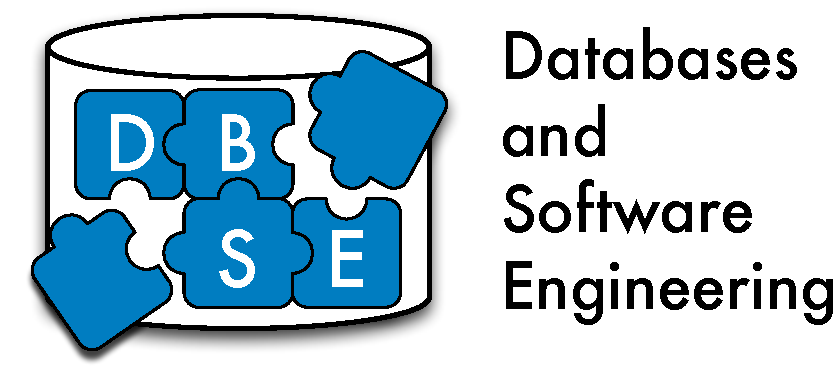
\includegraphics[scale=.35]{DBSE}}

\newcommand{\advisorone}{M.Sc.\ {Gabriel Campero Durand}}
\newcommand{\departmentone}{\ifgerman{Institut für}{Data and Knowledge Engineering Group}  }    
                               

\newcommand{\advisortwo}{Prof. Dr. rer. nat. habil. \ {Gunter Saake}}
\newcommand{\departmenttwo}{\ifgerman{Institut für}{Data and Knowledge Engineering Group}  }   

% Thesis kind
\ifgerman{\newcommand{\thesiskind}{Masterarbeit}}{\newcommand{\thesiskind}{Master's Thesis}}

\ifgerman{
	\newcommand{\theforename}{\todo{Vorname}}
	\newcommand{\thesurname}{\todo{Nachname}}
	\newcommand{\thetitle}{\todo{Titel der Arbeit}}
	\newcommand{\thedate}{\todo{13. Monat 2014}}
}{
	\newcommand{\theforename}{{Sameh}}
	\newcommand{\thesurname}{{Manaa}}
	\newcommand{\thetitle}{{Evaluation of Physical Structures for Graph Database Usage
}}
	\newcommand{\thedate}{{September 23, 2018}}
}
\newcommand{\theyear}{{2018}}

%*********************************************************************%
% SETUP                                                               %
%*********************************************************************%

% meta informations of the document
\hypersetup{
     pdfauthor={\theforename\ \thesurname},
     pdftitle={\thetitle}
}
% open index file
\ifnotdraft{\makeindex}

%*********************************************************************%
% ACRONYMS                                                            %
%*********************************************************************%

% HOWTO: \gls{IDE} for singular or \glspl{IDE} for plural with 's
%\makeglossaries
\newacronym{IDE}{IDE}{Integrated Development Environment}
%\glsaddall % use only if you have acronyms that occur only in graphics

%*********************************************************************%
% THE DOCUMENT                                                        %
%*********************************************************************%
\pgfplotsset{compat=1.14}

\usepackage{subfigure}
\usepackage{multirow}
\usepackage{lscape}
\usepackage{longtable}



\begin{document}

\ifgerman{
	\labelformat{lstlisting}{Quelltext~#1}
	\renewcommand{\lstlistingname}{Quelltext}
}{
	\labelformat{lstlisting}{Listing~#1}
}

% set the path where graphics are located
\graphicspath{{pics/}}

\ifnotdraft{
	\frontmatter
	\pagenumbering{roman}
	\newcommand{\theauthor}{\theforename\ \thesurname}
\newcommand{\theauthorr}{\thesurname,\ \theforename}
\begin{titlepage}
 \thispagestyle{empty}
 \begin{center}
  {\university}\\[0.4cm]
  {\school}\\[0.8cm]
   \hbox{}\hfill
    \begin{minipage}[t]{\textwidth}
      \begin{center}
        \logo\ifdbse{\\[0.4cm]
        \logodbse
        }{ }
      \end{center}
    \end{minipage} 
   \hfill\hbox{}
  \ \\[0.4cm]
  \ifdbse{
  {\large \thesiskind \\[1cm]}
  {\huge\bf \thetitle \\[1cm]}
  }
  {
  {\large \thesiskind \\[1.4cm]}
  {\huge\bf \thetitle \\[1.6cm]}
  }
  { \ifgerman{Autor:}{Author:}}\\[0.3cm]
  {\huge \theauthor}\\[0.8cm]
  {\large\thedate}\\[0.8cm]
  {\ifgerman{Betreuer:}{Advisors:}}\\[0.3cm] 
  {\large
\advisorone
  }\\[0.2cm]
  {
\departmentone
  }\\[0.8cm]
  {\large
\advisortwo\ 
  }\\[0.2cm]
  {
\departmenttwo\ 
  }\\[0.8cm]
 \end{center}
\end{titlepage}

%%%%%%%%%%%%%%%%%%%%%%%%%%%%%%%%%%%%%%%%%%%%%%%%%%%%%%%%%%%%%%%%%%%%%%%%%%%%
%%% Titelrückseite: Bibliographische Angaben
%%%%%%%%%%%%%%%%%%%%%%%%%%%%%%%%%%%%%%%%%%%%%%%%%%%%%%%%%%%%%%%%%%%%%%%%%%%%

\thispagestyle{empty}
\vspace*{\fill}
\begin{minipage}{15.0cm}
\textbf{\theauthorr:}\\
\emph{\thetitle\\}
\thesiskind, \university, \theyear.
\end{minipage}
\newpage

	\ifgerman{\chapter*{Inhaltsangabe}}{\chapter*{Abstract}}

Graph database management systems have emerged as specialized databases that can store and process relationships among the data entities in an efficient way. Graph databases are equipped with many components that work together in order to handle even the very complex relationships that can exist in a network of connected data. One of the main components of a graph database is its storage system. The storage system of a graph database is utilizing a set of graph data structures in order to efficiently manage the storage of graph data. 

For the construction of a graph storage system; many graph data structures are available as alternatives to choose from. Each graph data structure has its unique way in representing graph data. The different representations of graph data implies a difference in the complexity of the data storage and retrieval operations performed on each of the graph data structures. Choosing the right graph data structure for the storage of graph data is challenging without a comprehensive benchmarking of the many available graph data structures.

In this thesis, we study a set of graph data structures concerning the way they represent the graph data stored from the logical and physical perspectives. We evaluate the performance of the graph data structures according to a set of well-defined dimensions. Our evaluation of the graph data structures is based on an in-memory implementation of the data structures. 

By the end of this thesis, we will provide answers for a set of evaluation questions concerning the scalability, loading, and query performance of a set of graph data structures. We believe the answers to those questions will aid graph database designers in their choices for the graph data structure to use.

{\chapter*{Acknowledgements}}

It is a pleasure to finally get this work done. I would like to thank my advisors Prof. Gunter Saake, and M.Sc. Gabriel Campero Durand for their support, guidance, and supervision throughout my journey in writing this thesis. 

Also, I would like to thank my family and friends for the continuous support, and encouragement they have shown me during my entire master's studies, and especially during my thesis writing.





{\chapter*{Declaration of Academic Integrity}}

I hereby declare that this thesis is solely my own work and I have cited all external sources used.

\textit{Magdeburg, November 19th 2018} 



\begin{flushright}
\textbf{——————–} \\
\textbf{Sameh Manaa}
\end{flushright}

	\blankpage




% 	\chapter*{Acknowledgements}
% 	\ldots
% 	\blankpage
}

%*********************************************************************%
% LISTINGS                                                            %
%*********************************************************************%

\ifnotdraft{
	{\parskip 0pt \pdfbookmark{\contentsname}{\contentsname}\chapterheadfont \tableofcontents} % toc bitte einzeilig
	\blankpage

	\ifgerman{
		\listoffigures
		\addcontentsline{toc}{chapter}{Abbildungsverzeichnis}

		\listoftables
		\addcontentsline{toc}{chapter}{Tabellenverzeichnis}

		\renewcommand{\lstlistlistingname}{Quelltextverzeichnis}
		\blankpage
		\lstlistoflistings
		\addcontentsline{toc}{chapter}{\lstlistlistingname}

		%\renewcommand*{\firstacronymfont}[1]{\emph{#1}}
		%\printglossary[type=acronym,title=List of Acronyms,toctitle=Abkürzungsverzeichnis]
	}{
		\listoffigures
		\addcontentsline{toc}{chapter}{List of Figures}

% 		\listoftables
% 		\addcontentsline{toc}{chapter}{List of Tables}

% 		\renewcommand{\lstlistlistingname}{List of Code Listings}
% 		\blankpage
% 		\lstlistoflistings
% 		\addcontentsline{toc}{chapter}{\lstlistlistingname}

		%\renewcommand*{\firstacronymfont}[1]{\emph{#1}}
		%\printglossary[type=acronym,title=List of Acronyms,toctitle=List of Acronyms]
	}
}

%*********************************************************************%
% CHAPTERS                                                            %
%*********************************************************************%

\mainmatter
\pagenumbering{arabic}

{\chapter{Introduction}
\label{chap:Introduction}

%(a) State the problem to be solved.
Graph databases are characterized by being able to store and query a network of connected data with a performance that exceeds other non-graph databases (e.g. relational databases). Graph databases are flexible in modeling graph data, allowing for the evolve of the model by adding new vertices, edges, or properties as demanded without compromising the stability or performance of the system. Native graph databases differentiate themselves from non-native graph databases by using data structures that are specifically designed for the storage of graph data, in contrast to the use of other kinds of databases as the back-end storage system which is the case in the non-native graph databases \cite{robinson2013graph}. 

In a survey performed by (\textit{Sahu et al.}), many participants have reported the use of graph databases to store and process graph data that is huge in size (more than 1 billion edge). The participants in the survey have reported a wide variety of computations that they perform on the stored data. The computations the users performed ranged from simple traversal queries and up to complex analytical queries. However, the survey participants have reported the scalability of the database to manage bigger sizes of data and perform more complex computations as their top challenge. Loading graph data or performing traversal queries are considered a very time consuming operations when done on a graph with large size \cite{sahu2017ubiquity}.

The scalability and query performance issues of a graph database are indicators of the difficulties that the database is facing in order to handle the growing data size. A major part of the performance of a graph database lies in the ability of its storage system to accommodate graph data with larger size without hindering the accessibility of the data. The design choices of the storage system include the proper choice of a graph data structure for the storage of graph data. Each graph data structure is representing graph data in a distinct way and hence the difference in the performance of each graph data structure in storing new data or reaching existing ones.\\

%(b) Discuss the state of the art (i.e., previous work) and explain why, despite/because of this literature, there remains: (i) confusion; (ii) misunderstanding; (iii) errors; or (iv) some unresolved problem. Alternatively, present an empirical puzzle that the existing literature fails to explain.

Few work has been done on evaluating the alternative choices of graph data structures which will aid graph database designers in choosing the proper graph data structure that fits the user requirements. Current work done in this area has only evaluated a subset of the available graph data structures. In their work, \textit{(Wheatman et al.)} have evaluated only adjacency list and compressed sparse row (CSR) performance in loading and query performance leaving out other graph data structure like adjacency matrix \cite{wheatmanpacked}. Other work done by \textit{(Then et al.)}, has evaluated various techniques of parallel graph loading \cite{then2016evaluation}. \\

Both work \cite{wheatmanpacked, then2016evaluation} have presented evaluation of loading and querying of graph topology structures which are used to represent the edges between the graph vertices. We found no previous work on evaluating the performance of graph properties structures such as (universal table, emerging schema, or nested key-value store) against each other. Graph properties structures are used to represent the properties associated with each graph element (vertices and edges) in the property graph model. The property graph model (PGM) is the most widely implemented graph data model in graph databases. Also, we found no work that covers the evaluation of graph data structures in the presence of a multi-graph data. The multi-graph property allows more than one edge between the same two vertices. Multi-graphs and graph properties are two important characteristics of the property graph model \cite{robinson2013graph}. Lastly, we found no work that evaluates the performance of graph data structure when loaded in batches of data neither the impact of the batch-size on the performance of the loading process.\\


%(c) State the essence of your contribution, that is, your solution to the problem or puzzle. Give the reader a sense of how you will solve the problem; provide some confidence that if she reads the rest of your paper, she has a chance of learning something.


In this thesis, we aim to present a comprehensive evaluation of the major graph data structures that have been developed specifically for the storage and processing of graph data. Our contribution in this thesis is summarized in the following points:


\begin{itemize}  
\item\textbf{Graph Data Structures:}\\
We study the major available graph data structures from two perspectives. First, we study the graph structures logical design and the characteristics of each graph structure. Next, we present our physical design of the different graph structures which we have constructed using the data structures offered as part of the \textit{Standard Template Library} (STL) of the $C++$ programming language. For evaluation purposes, we implement all the data structures for in-memory processing of data with no involvement of disk persistent storage.\\

\item \textbf{Scalability of Graph Structures:}\\
We present an extensive evaluation of the scalability of the different graph structures. We evaluate the scalability of a graph structure by measuring the amount of memory storage as well as the time taken to store graph data. We use a different sizes of a graph dataset generated by the \textit{LDBC} benchmarking framework \cite{boncz2013ldbc}.\\

\item \textbf{Evaluation of Loading Techniques:}\\
We present an evaluation of two techniques for graph data loading. First, we evaluate a batch loading technique and the impact of the batch-size on the performance of the loading process. Next, we evaluate a parallel loading technique and the change in data loading time that loading the data in parallel could introduce in comparison to sequential loading.\\

\item \textbf{Evaluation of Query Execution:}\\
We present the definition of a set of queries which compute centrality or perform pattern-matching on the loaded graph data. We evaluate the time taken to execute each of the given queries on the data loaded in each of the graph structures.

\end{itemize}


%(d) The last paragraph of your introduction should always be a "road map" paragraph; for example: "This paper proceeds as follows. In section 1 ..."

The thesis is consisted of the following chapters: 

\begin{itemize}  
\item\textbf{Background:}\\
In (\ref{chap:Background}), we present the necessary background knowledge concerning topics covered in this thesis.

\item \textbf{Physical Design of Graph Data Structures:}\\
In (\ref{chap:PhysicalDesign}), we present the set of evaluation questions we are going to answer in this thesis as well as the physical design of the graph data structures, we are going to evaluate.

\item \textbf{Evaluation Environment:}\\
In (\ref{chap:Eval_4}), we introduce the details of every component in the evaluation environment which we will use to evaluate our implemented graph data structures.

\item \textbf{Evaluation: Scalability and Data Loading:}\\
In (\ref{chap:Eval_5}), we present the first part of the evaluation results for the experiments we conducted on the graph data structures concerning the scalability of the graph structures and the performance of data loading.

\item \textbf{Evaluation: Queries:}\\
In (\ref{chap:Eval_6}), we present the second and last part of the evaluation results for the experiments we conducted to evaluate the performance of the graph structures in query execution scenarios.

\item \textbf{Related Work:}\\
In (\ref{chap:RelatedWork}), we present work by other researchers which we see as related to the work done in this thesis.

\item \textbf{Conclusion and Future Work:}\\
In (\ref{chap:Conclusion}), we draw a conclusion of the thesis as well as suggesting research points that can be a further extension of our work.  
\end{itemize}


}
{\chapter{Background}
\label{chap:Background}

In this chapter, we present the necessary background knowledge concerning topics covered in this thesis. This chapter is consisted of the following sections: 

\begin{itemize}  
\item\textbf{Graphs:}\\
In (\ref{sec:Graphs}), we make a definition for a graph according to the graph theory and discuss the different graph types.

\item \textbf{Graph Data Models:}\\
In (\ref{sec:GraphModels}), we discuss the property graph model (PGM) and the resource description framework model (RDF), as two types of logical graph data models that are mostly used by state of the art graph databases.

\item \textbf{Graph Data Structures:}\\
We present the data structures used by graph databases for the storage of graphs in (\ref{sec:StorageStructures}).

\item \textbf{Summary:}\\
Lastly, we make a summary of the main topics we discussed in this chapter in (\ref{sec:BackgroundSummary}).
\end{itemize}

\section{Graphs}
\label{sec:Graphs}
In this section, we discuss graphs and graph  types. In (\ref{subsec:Graph?}), we adopt a clear definition for graphs. A definition that is based on the graph theory. In (\ref{subsec:GraphTypes}), we state the different types of graphs. A graph type is a factor that must be taken into consideration in the storage and retrieval methods of the graph.

\subsection{What is a Graph?}
\label{subsec:Graph?}
Graph theory is a mathematical topic that is focused on the study of graphs. A graph \textit{G = (V,E)} is defined as a finite nonempty set \textit{V} of vertices along with the set \textit{E} of edges. The set \textit{E} consists of unordered pairs of vertices in \textit{V}, where an edge \textit{x \(\in\) E} is defined as a pair of vertices \(\textit{x = \{u,v\}}\) \cite{harary6graph}.

We define any two vertices $u \in V$ and $v \in V$ that forms any of the edges in \textit{E} as adjacent vertices. Similarly, two edges $x \in E$ and $y \in E$ are adjacent if they are formed of two pair of vertices where the two pair are sharing one common vertex. The adjacencies of a vertex \textit{u}, is the set $K \subset V$ of vertices, where for each vertex $a \in K$, there is an edge \mbox{$s \in E$} and \textit{s = \{u,a\}} \cite{harary6graph}.

\begin{figure}
\centering
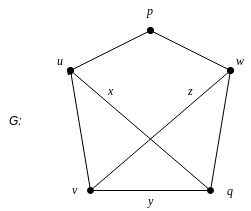
\includegraphics[width=10cm]{pics/Graph.png}
\caption{An example of a graph \textit{G} \cite{harary6graph}.}
\label{fig_graph}
\end{figure} 

In (\ref{fig_graph}), we are showing an example of a graph \textit{G}. In graph \textit{G}, vertices \textit{u} and \textit{v} are adjacent while vertices \textit{u} and \textit{w} are not. Similarly, edges \textit{x} and \textit{y} are adjacent while edges \textit{x} and \textit{z} are not. The adjacencies of vertex \textit{u} in the graph is the set of vertices \textit{\{p,v,q\}} \cite{harary6graph}.




\subsection{Graph Types}
\label{subsec:GraphTypes}

Graphs come in many types and shapes according to how rich they are with information. In (\ref{fig_graph-types}), we show an example of different graph types. A short explanation of each graph type is included in the below list. Some of the below mentioned graph types can be be used together to form one graph \cite{DBLP:journals/corr/abs-1006-2361}.
\\
\\

\begin{figure}
\centering
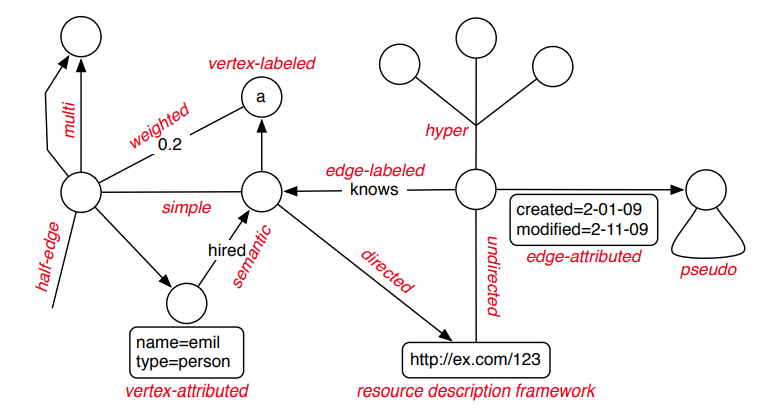
\includegraphics[width=17cm]{pics/graph-types.png}
\caption{An example of different graph types \cite{DBLP:journals/corr/abs-1006-2361}.}
\label{fig_graph-types}
\end{figure} 

\begin{itemize}  
\item \textbf{Simple Graph:} a graph that permits no loops and only binary edges are allowed.

\item \textbf{Multi-graph:} a graph that allows the existence of more than one edge connecting the same two vertices.

\item \textbf{Pseudo Graph:} a graph with reflexive edges

\item \textbf{Weighted Graph:} a graph where a weight is assigned to edges to show the relationship strength.

\item \textbf{Semantic Graph:} used in semantic networks to model the relationships between concepts.

\item \textbf{Half-edge Graph:} an edge that is connected at one of its two ends to a vertex and on the other end connected to nothing.

\item \textbf{Hyper-graph:} a graph that permits an edge to connect more than one vertex.

\item \textbf{Directed Graph:} a graph where each edge is defined by an ordered pair of vertices (one of them is a source vertex and the other is a target vertex).

\item \textbf{Undirected Graph:} a graph where edges are denoting symmetric relationships between edges.

\item \textbf{Edge-labeled Graph:} used to specify the kind of relationship between vertices.

\item \textbf{Vertex-labeled Graph:} a graph where a label is assigned to a vertex to describe the vertex's type or set the vertex's identity.

\item \textbf{Edge-attributed Graph:} a graph where descriptive properties are assigned to edges.

\item \textbf{Vertex-attributed Graph:} a graph where descriptive properties are assigned to vertices.

\item \textbf{Resource Description Framework (RDF) Graph:} a graph where vertices and edges are identified by Uniform Resource Identifiers (URI). The RDF is a standard that was issued by the World Wide Web consortium.

\end{itemize}


\section{Graph Data Models}
\label{sec:GraphModels}

In (\ref{sec:Graphs}), we presented the definition of graph and introduced the difference between the various graph types. In this section, we discuss two logical graph data models. First, we present the property graph model (PGM) in (\ref{subsec:PGM}). Next, we present the resource description framework model (RDF) in (\ref{subsec:RDF}).


\begin{figure}[H]
\centering
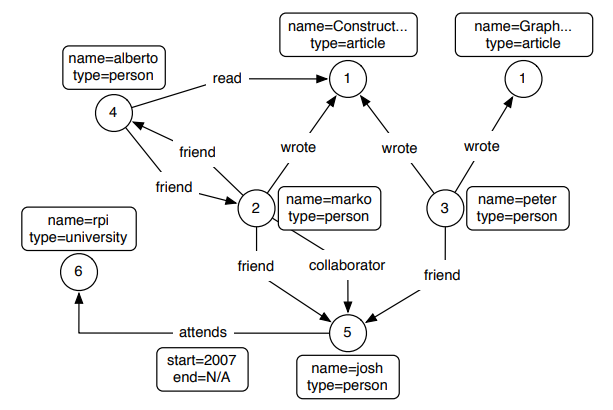
\includegraphics[width=17cm]{pics/PGM.png}
\caption{A diagram of a property graph \cite{DBLP:journals/corr/abs-1006-2361}.}
\label{fig_PGM}
\end{figure} 

\subsection{Property Graph Model}
\label{subsec:PGM}

Several graph database systems are supporting the property graph model. The property graph model is characterized with being directed, labeled, attributed and multi-graph. In (\ref{fig_PGM}), we show an example diagram of a property graph model. 

In property graph model, an edge is defined as an ordered pair of vertices. The first vertex in the pair is the source vertex of the edge and the second vertex in the pair is the target vertex of the edge. 

Vertices and edges in a property graph model are labeled. A vertex label is an identifier for the vertex while an edge label is used to define the relationship type of an edge. 

A vertex in the property graph model is described by properties (or attributes). The properties describing a vertex are a set of key-value pairs. An example of a property describing a vertex in (\ref{fig_PGM}) is \textit{"name"="alberto"} property which is describing vertex "4". Similarly, an edge can also be described by a set of key-value properties. An example of a property describing an edge in (\ref{fig_PGM}) is \textit{"start"="2007"} property which is describing edge "attends".

Property graph model is supporting also the creation of multi-graphs. In a multi-graph, more than two edges can be defined using the same pair of vertices and with the same direction, given that the edges have different labels \cite{DBLP:journals/corr/abs-1006-2361, Robinson:2015:GDN:2846367}.



\subsection{Resource Description Framework Model (RDF)}
\label{subsec:RDF}

The World Wide Web consortium (W3C) has developed the Resource Description Framework (RDF) as a foundation for metadata exchanging and processing across the web. RDF is used mostly in building semantic webs. The RDF standard is used to express the metadata of the web documents. RDF is well supported by a model of triples. A triple is consisting of a resource, a property, and a value. The RDF model is characterized with being a vertex-labeled, edge-labeled, and directed graph \cite{ngomo2014introduction}.

A resource is anything that can be uniquely identified using a Unique Resource Identifier (URI). A web page is an example of a resource identified by its Unique Resource Locator (URL). A property is used to define a binary relationship between a resource and a value. A value itself can be a resource or a string of characters. A triple is considered as an RDF statement that is defined by the three elements (resource, property, value) \cite{Las99,Lee2005}.



In (\ref{fig_RDF}), we show an example of an RDF graph that is consisting of 9 triples. The graph is describing the city of Leipzig and its mayor. An example of a triple in the graph is \textit{("Leipzig", "locatedIn", "Saxony")} with \textit{"Leipzig"} representing the resource, \textit{"locatedIn"} representing the property, and \textit{"Saxony"} representing the value in the triple.


\begin{figure}[H]
\centering
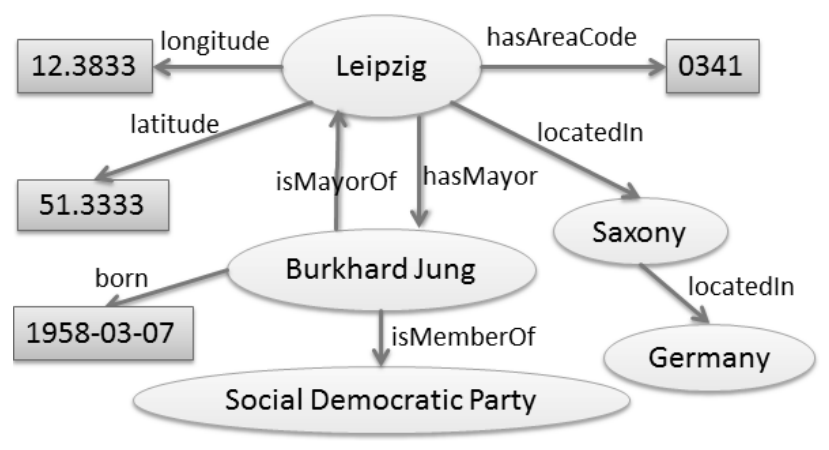
\includegraphics[width=15cm]{pics/RDF-Graph.png}
\caption{An example of an RDF graph that consists of 9 triples \cite{ngomo2014introduction}.}
\label{fig_RDF}
\end{figure} 

\section{Graph Data Structures}
\label{sec:StorageStructures}

In (\ref{sec:GraphModels}), we presented two logical graph data models. First, we presented the property graph model (PGM) in (\ref{subsec:PGM}). Next, we presented the resource description framework model (RDF) in (\ref{subsec:RDF}). In \cite{Paradies2017},  the authors (\textit{Paradies et al.}) have categorized the data structures used to store graph data into two categories. First category is for the graph data structures used by graph databases for solely storing a directed graph topology. Second category is for the graph data structures used by graph databases for solely storing graph properties. In this section, we adopt the categorization presented in \cite{Paradies2017} and present the necessary background information of a selected subset of graph data structures. We first discuss three data structures (Adjacency Matrix, Compressed Sparse Row (CSR), Adjacency List) for graph topology in (\ref{subsec:GraphTopology}). Next, we present three data structures (Universal Table, Emerging Schema, Nested Key-Value Store) for storing graph properties in (\ref{subsec:GraphProperties}).


\subsection{Graph Topology}
\label{subsec:GraphTopology}

The graph topology storage structures are meant to store the topology of a graph. We mean by the topology of a graph, the vertices of the graph identified by their labels and the directed edges connecting those vertices, leaving out the edge-labels, vertex-properties and edge-properties.

In this section, we introduce three data structures that can be utilized by graph databases for the storage of a graph topology. In (\ref{subsubsec:AdjacencyMatrix}), we present the adjacency matrix as the first storage structure for graph topology. Next, we present the compressed sparse row (CSR) in (\ref{subsubsec:CSR}). Lastly, we present the adjacency list in (\ref{subsubsec:AdjacencyList}).


\begin{figure}[H]
\centering
    \subfigure[Directed graph \textit{G}.]
    {
        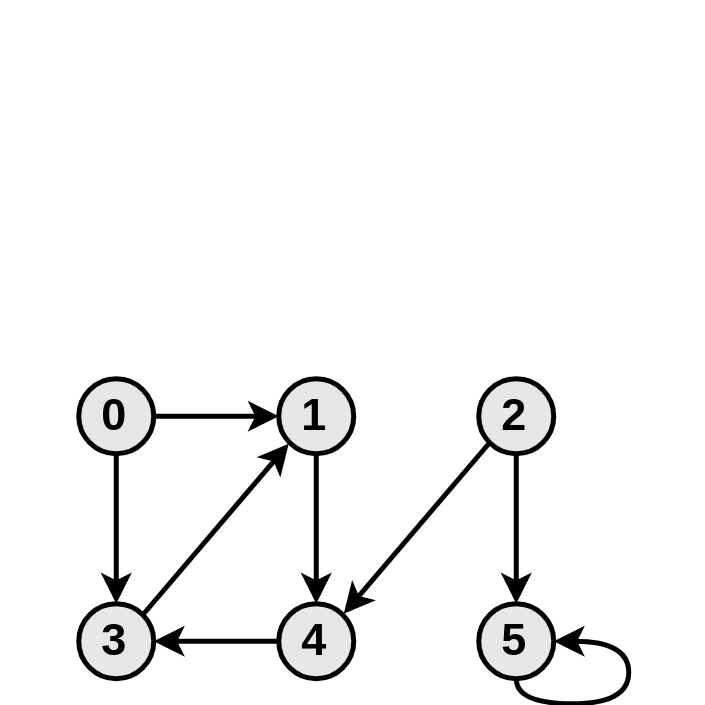
\includegraphics[width=0.35\textwidth]{pics/DirectedGraph.png}
        \label{fig:directedGraph_logical}
    }
\centering
    \subfigure[Adjacency matrix representation of \textit{G}.]
    {
        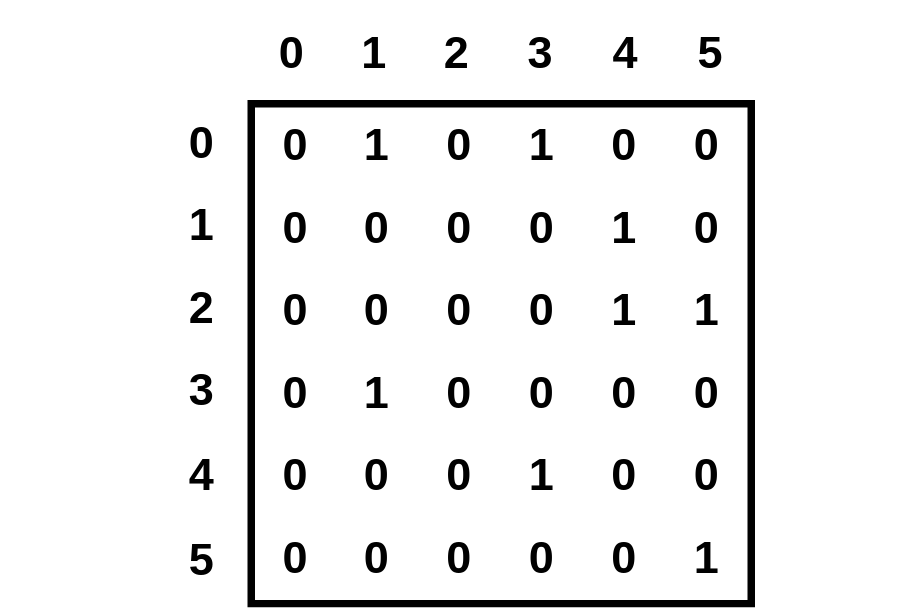
\includegraphics[width=0.42\textwidth]{pics/AdjacencyMatrix_logical.png}
        \label{fig:adjMat_logical}
    }
    \\
\centering
    \subfigure[CSR representation of \textit{G}.]
    {
        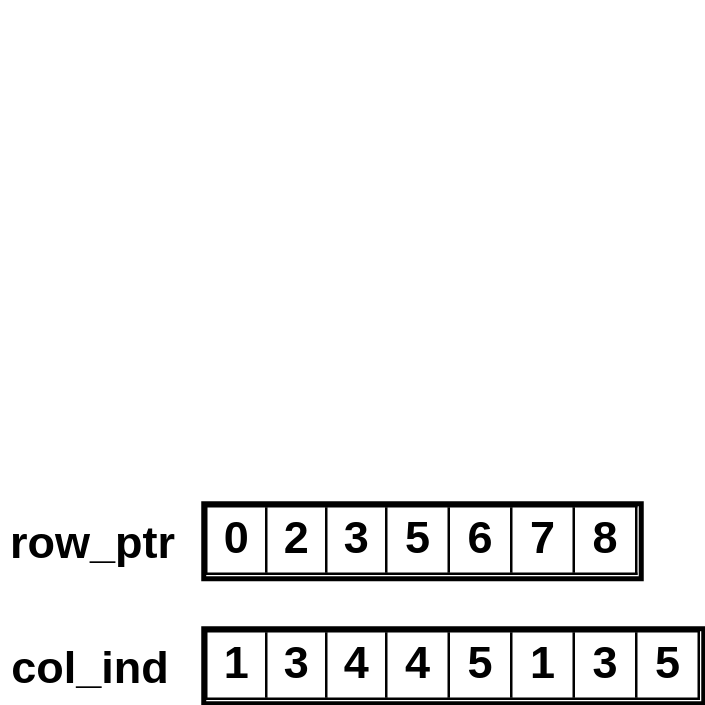
\includegraphics[width=0.35\textwidth]{pics/CSR_logical.png}
        \label{fig:CSR_logical}
    }
    \subfigure[Adjacency list representation of \textit{G}.]
    {
        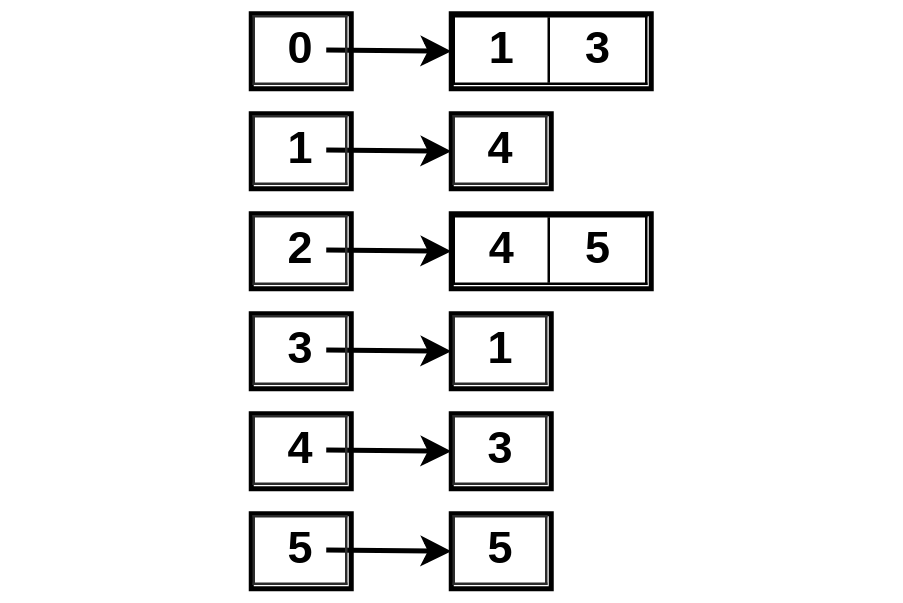
\includegraphics[width=0.4\textwidth]{pics/AdjacencyList_logical.png}
        \label{fig:adjLst_logical}
    }
    \caption{Logical representations of the topology of directed graph \textit{G} \cite{cormen2009introduction}.}
    \label{fig:GraphTopology_logical}
\end{figure}


\subsubsection{Adjacency Matrix}
\label{subsubsec:AdjacencyMatrix}

The adjacency matrix is the preferred method of storing graph \textit{G = (V,E)} when the graph is dense (i.e. \textit{$|E| \approx |V|^2$}) or in case there is a need to get a fast response on checking for two vertices \textit{u} and \textit{v}, if there is an edge tying them to each other. 

For a directed graph \textit{G = (V,E)}, the adjacency matrix \textit{A} representing the graph is a \textit{$|V| \times |V|$} matrix and the vertices of the graph are labeled with a sequence of numbers 1,2,...,\textit{|V|}. For a cell \textit{$a_{ij}$} in matrix \textit{A} where \textit{$1 \leq i \leq |V|$} and similarly \textit{$1 \leq j \leq |V|$}, a value of "1" is assigned to the cell if \textit{(i,j) \(\in\) E}, otherwise, a value of "0" is assigned to the cell \cite{cormen2009introduction}.

In (Figure \ref{fig:directedGraph_logical}), we show an example of a directed graph \textit{G} that is consisted of 6 vertices and 8 edges. In (Figure \ref{fig:adjMat_logical}), we show the adjacency matrix logical representation of \textit{G} \cite{cormen2009introduction}. 

The memory required for storing an adjacency matrix of a graph is $O(|V|^2)$ which is not affected by the number of edges \textit{|E|} in the graph \cite{cormen2009introduction}.



\subsubsection{Compressed Sparse Row (CSR)}
\label{subsubsec:CSR}

Sparseness of an adjacency matrix \textit{A} can be solved by storing only the non-zero elements of the matrix (i.e. recording only the existence of an edge and discarding information about the absence of an edge between two vertices). The compressed sparse row (CSR) is a compact storage format that stores only non-zero elements of a sparse matrix. The compressed sparse row (CSR) format is storing the information about the non-zero elements of the matrix in two vectors with contiguous memory locations \textit{(col\_ind,row\_ptr)}. We store the column indices of the non-zero elements in the matrix in \textit{col\_ind} ordered by their position precedence in the matrix when scanning the matrix in a row-wise left-to-right traversal. In \textit{row\_ptr}, we store only the indices of the elements in \textit{col\_ind} that are located first in their respective rows in the matrix \cite{Bai:2000:TSA:357352,Paradies2017}.

In (Figure \ref{fig:CSR_logical}), we show the compressed sparse row (CSR) that is representing the adjacency matrix in (Figure \ref{fig:adjMat_logical}) and consequently representing the directed graph \textit{G} in (Figure \ref{fig:directedGraph_logical}) \cite{Bai:2000:TSA:357352}.

Instead of storing $|V|^2$ elements in the adjacency matrix, the compressed sparse row (CSR) format is consuming much less storage by storing only $nnz + |V| + 1$ elements, where $nnz$ is the number of non-zero elements in the matrix \cite{Bai:2000:TSA:357352}. Although the compressed sparse row (CSR) format is offering a contiguous memory allocation of the graph data compacted in two vectors, a manipulation by adding or removing elements to CSR is expensive. Because the order of elements stored in the two vectors \textit{(col\_ind,row\_ptr)} must always be maintained, a manipulation to the CSR data implies a reorganization of the elements in the vectors to maintain their elements order.

\subsubsection{Adjacency List}
\label{subsubsec:AdjacencyList}

In adjacency matrix we have faced the problem of storing redundant and unnecessary information regarding the absent edges. Although the compressed sparse row (CSR) format has offered a solution to this problem by storing only the necessary information, it raised a different issue which is the expensive manipulation of the data.

The adjacency list \textit{Adj} of a graph \textit{G = (V,E)} is composed of a set of $|V|$ pairs. Each pair is consisted of a vertex $u$ and a vector $K$ that contains the adjacencies of $u$ \cite{van1998python}.

Adjacency lists is memory efficient in storing sparse graphs by storing only information that indicates the existence of an edge. Adjacency lists keeps the adjacencies vector $K$ of each vertex ordered for efficient look-up operations. Adding or removing a vertex to/from $K$ requires a reorganization of the elements in the vector to maintain the elements order. The overhead of reorganizing the elements in $K$ is proportional to the size of $K$ which is less when compared to the similar overhead in CSRs that is proportional to $|V|$ \cite{van1998python}.

In (Figure \ref{fig:directedGraph_logical}), we show an example of a directed graph \textit{G} that is consisted of 6 vertices and 8 edges. In (Figure \ref{fig:adjLst_logical}), we show the adjacency list logical representation of \textit{G} \cite{cormen2009introduction}. 

The memory required for storing an adjacency list of a graph is $O(|V| + |E|)$ \cite{cormen2009introduction}.







\begin{figure}[H]
\centering
    \subfigure[An attributed property graph \textit{G}.]
    {
        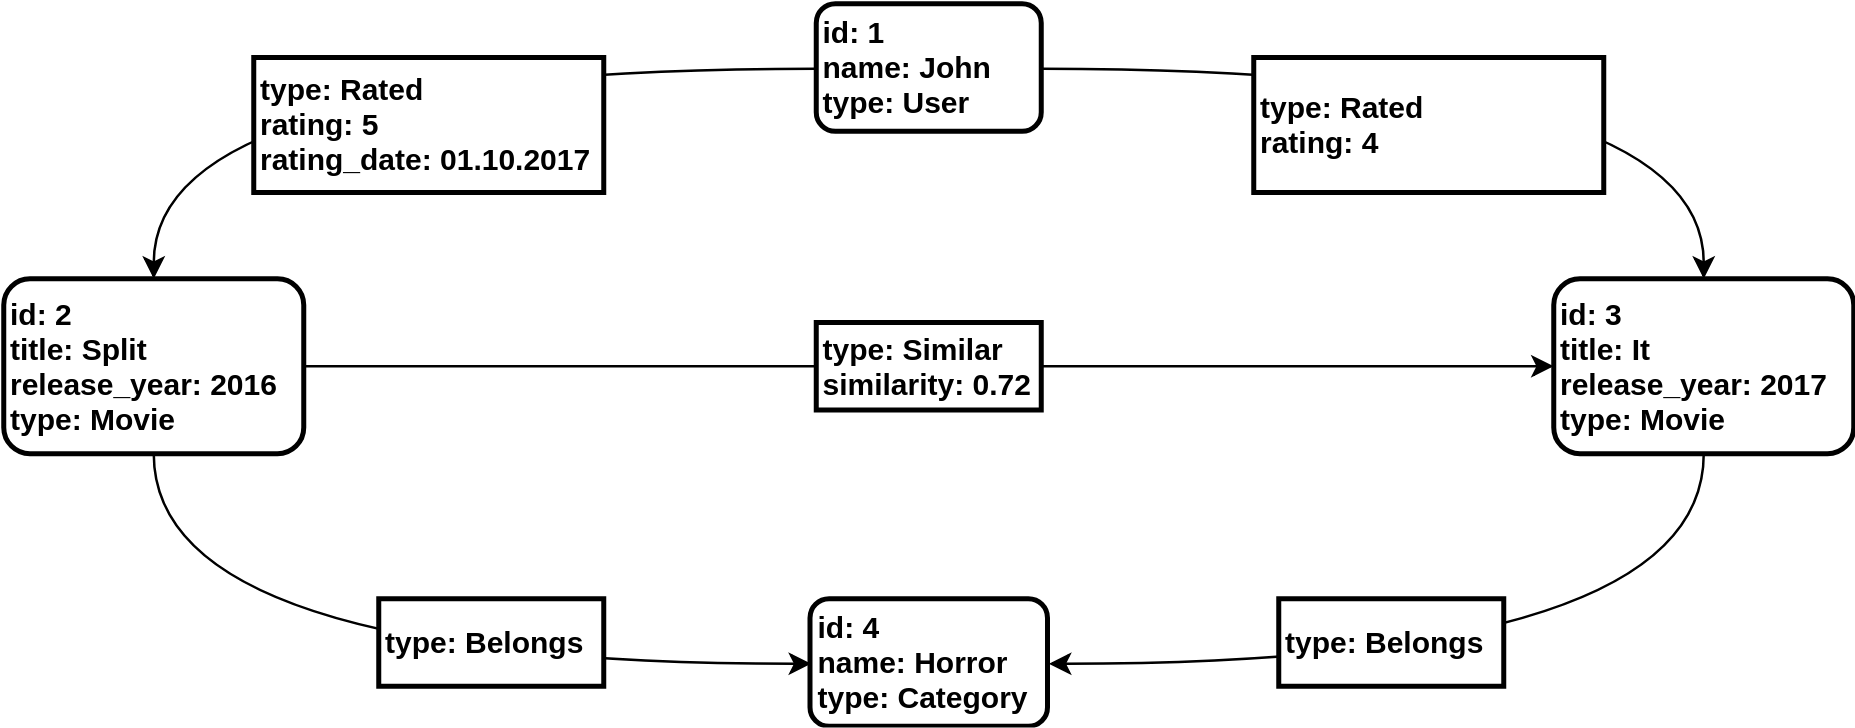
\includegraphics[width=1\textwidth]{pics/PropertyGraph.png}
        \label{fig:PropertyGraph}
    }
\centering
    \subfigure[Vertex universal table of \textit{G}]
    {
        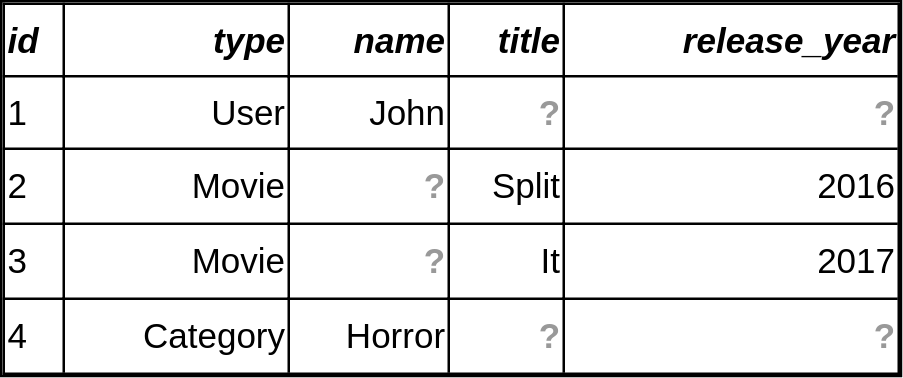
\includegraphics[width=0.45\textwidth]{pics/VertexUniversalTable.png}
        \label{fig:VertexUniTbl}
    }
\centering
    \subfigure[Edge universal table of \textit{G}.]
    {
        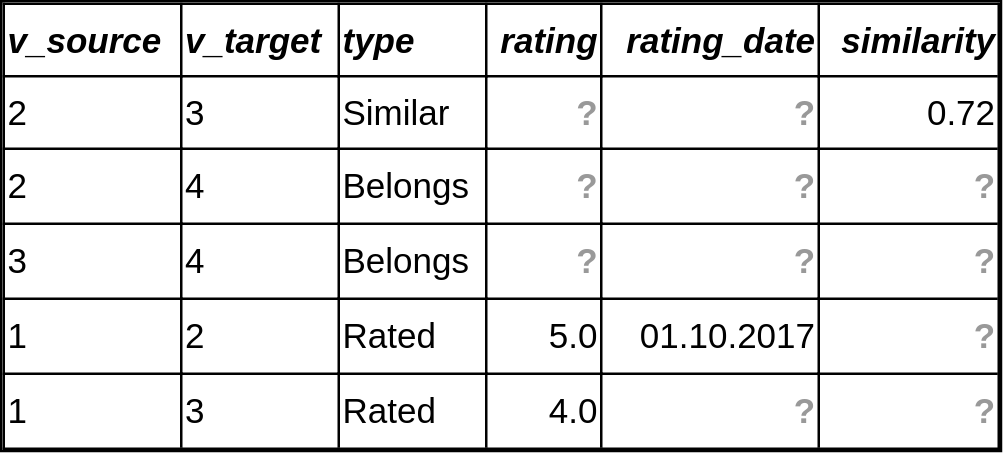
\includegraphics[width=0.5\textwidth]{pics/EdgeUniversalTable.png}
        \label{fig:EdgeUniTbl}
    }
\centering
    \subfigure[Emerging Schema - vertex column groups of \textit{G}.]
    {
        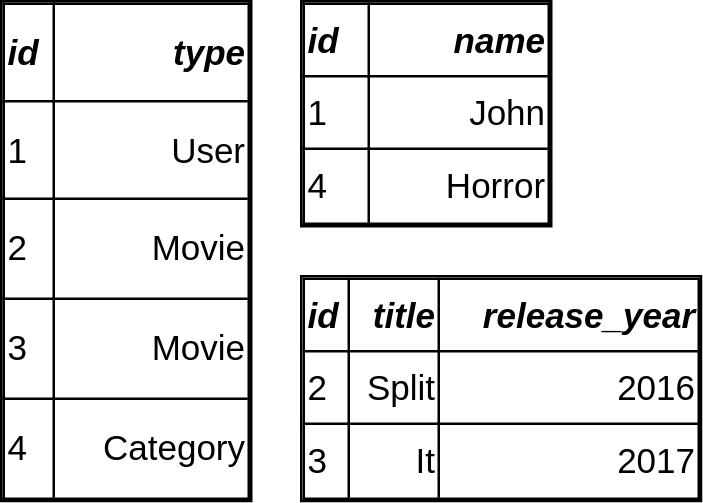
\includegraphics[width=0.45\textwidth]{pics/VertexEmergingSchema.png}
        \label{fig:VertexEmergingSchema}
    }
\centering
    \subfigure[Emerging Schema - edge column groups of \textit{G}.]
    {
        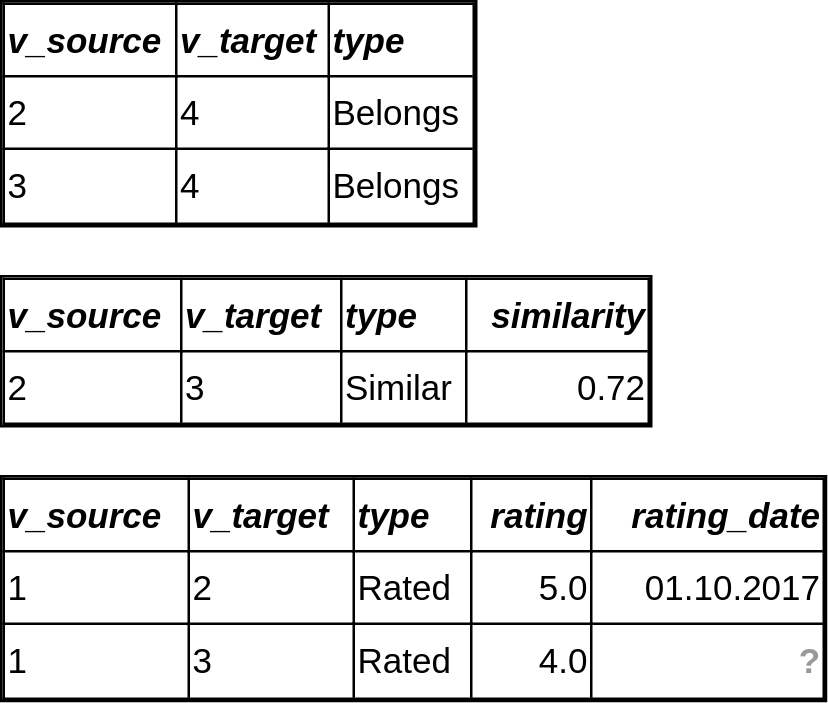
\includegraphics[width=0.5\textwidth]{pics/EdgeEmergingSchema.png}
        \label{fig:EdgeEmergingSchema}
    }
    \caption{Universal table and emerging schema representations of a property graph \textit{G}. \cite{DBLP:journals/corr/ParadiesLB14}.}
    \label{fig:GraphProperties_logical}
\end{figure}

\subsection{Graph Properties}
\label{subsec:GraphProperties}

In (\ref{subsec:GraphTopology}), we have introduced three graph topology data structures. The three data structures are storing information only regarding the graph topology, leaving out the storage of information regarding the properties of the graph to the graph properties data structures. 

In this section, we introduce three data structures that can be utilized by graph databases for storing the properties of vertices and edges for a given graph. In (\ref{subsubsec:UniversalTable}), we present the universal table. Next, we present the emerging schema approach in (\ref{subsubsec:EmergingSchema}). Lastly, we present the nested key-value store in (\ref{subsubsec:NestedkeyValueStore}).

\subsubsection{Universal Table}
\label{subsubsec:UniversalTable}

Universal tables is a method of storing the vertices and edges properties in only two tables. Each vertex is represented by a single row in the vertex universal table. Similarly, each edge is represented by a single row in the edge universal table. A column in the universal table is representing a distinct object's property. For an object's row in a universal table, a null value assigned to one of the object's columns means that the property represented by this column is not applicable to that object \cite{Paradies2017}.

Vertices and edges can have a distinct high number of properties which only a few of those properties are applicable to a specific vertex or edge. The in-applicability of all properties to every vertex or edge leads to a degree of sparseness in the universal table \cite{Paradies2017}.

The storage of an object (vertex or edge) in a single row allow for a join-free method to extract an object's properties \cite{Paradies2017}.

In (Figure \ref{fig:PropertyGraph}), we show an example of a property graph $G$ that is composed of 4 vertices and 5 edges. In (Figure \ref{fig:VertexUniTbl}), we present a vertex universal table for $G$, where each single vertex in $G$ is represented by a single row and each distinct vertex property is represented by a separate column. Similarly, in (Figure \ref{fig:EdgeUniTbl}), we present an edge universal table for $G$, where each single edge in $G$ is represented by a single row and each distinct edge property is represented by a separate column \cite{Paradies2017}.


\subsubsection{Emerging Schema}
\label{subsubsec:EmergingSchema}

In (\ref{subsubsec:UniversalTable}), we have discussed a simple method of storing an attributed graph using only a pair of universal tables, a vertex universal table and an edge universal table. The universal table method is subject to one drawback as it tends to be more sparse as the number of distinct attributes increase.

Emerging schema is a method that applies vertical partitioning on the properties of vertices/edges in a way that reduces the sparseness of the data and at the same time doesn't require the joining of many tables to extract a single object's properties. The emerging schema method is exploring the inherent schema in the data to create a set of column groups for vertices and another set of column groups for edges. 

One column group is consisted of multiple columns where the first column is always representing the unique object's identifier. In addition to the object's identifier column, properties that co-occur frequently together are clustered into the same column group \cite{Paradies2017}.

The clustering of the property attributes into column groups can be done by applying machine learning clustering algorithms such as k-means \cite{Paradies2017}. The input to the clustering algorithm is the set of distinct columns from all vertices (or edges). Each attribute is considered an $n-dimension$ point, where $n$ is the number of vertices or edges to be clustered and the value for each dimension is "1" in case a non-null value and "0" in case of a null value.

In (Figure \ref{fig:PropertyGraph}), we show an example of a property graph $G$ that is composed of 4 vertices and 5 edges. In (Figure \ref{fig:VertexEmergingSchema}), we present the vertex column groups for $G$ that is produced by the emerging schema method. A single vertex in $G$ can be represented in more than one of the resulted vertex column groups. Similarly, in (Figure \ref{fig:EdgeEmergingSchema}), we present the edge column groups for $G$ that is produced by the emerging schema method. A single edge in $G$ can be represented in more than one of the resulted edge column groups \cite{Paradies2017}.


\subsubsection{Nested Key-Value Store}
\label{subsubsec:NestedkeyValueStore}

In this section, we are presenting another approach for solving the sparseness problem of universal tables discuss in (\ref{subsubsec:UniversalTable}).

Graph properties are composed of vertices-properties and edges-properties. The properties of a vertex/edge are consisted of key-value pairs that describe the vertex/edge. In a given vertex-attributed and edge-attributed graph $G = (V,E)$, for each vertex $u \in V$ and edge $x \in E$, a set $P$ of key-value pairs exists. Each key-value pair $(k,v) \in P$, is consisted of a property $k$ that describes the vertex/edge and a value $v$ that is assigned to $k$ \cite{ladwig2011cumulusrdf}.

Nested key-value stores are storing an object's (vertex or edge) properties in a two level nested key-value stores. The first level of the store is representing rows, where each object is stored in a row. The object's row is represented by a key-value pair, where the key is a unique identifier for the object and the value is itself a second level of a key-value store. The key-value store on the second level is to represent columns, where each object's property is stored in a column. Each column is represented by a key-value pair, where the key is the name of the property describing the object and the value is a string of characters \cite{ladwig2011cumulusrdf}.

A vertex is identified by a unique id  that is assigned to the vertex, while an edge is identified by the edge's source and target vertices as well as the edge label in the case of a multi-graph. We store the properties of the vertices in one nested key-value store separated from another nested key-value store that we use for the storage of the properties of the edges.


\begin{figure}[t]
\centering
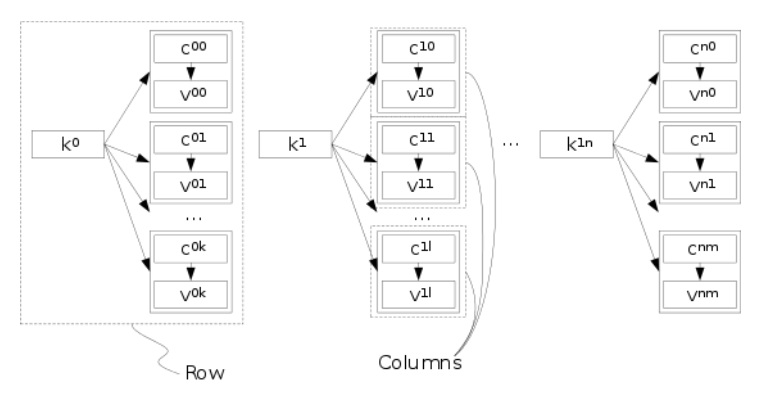
\includegraphics[width=15cm]{pics/NestedKey-ValueStore.png}
\caption{A nested key-value store composed of rows and columns \cite{ladwig2011cumulusrdf}.}
\label{fig_nestedKey-ValueStore}
\end{figure} 

In (\ref{fig_nestedKey-ValueStore}), we show a diagram of a nested key-value store that is composed of rows and columns. On the first level of the store rows are stored while columns are stored in the second level of the store \cite{ladwig2011cumulusrdf}.

The nested key-value store is searched for an object's row using the object's identifier $(k)$ and the value returned is the object's columns $(c)$. The object's columns $(c)$ are searched for a specific column or property to return the value $(v)$ of that column \cite{ladwig2011cumulusrdf}.




%\section{Data Structures in C++}
%\label{sec:DataStructuresInC++}

%\subsection{Vector}
%\subsection{Map}
%\subsection{Unordered Map}

\section{Summary}
\label{sec:BackgroundSummary}

In this chapter, we made a formal definition of a graph according to the graph theory and discussed the different graph types. We presented two logical graph models that are most commonly used  by state of the art graph databases, the property graph model (PGM) and the resource description framework model (RDF). We presented several storage structures used by graph databases to store graph data and we differentiated between structures used to store graph topology and structures used to store graph properties.

Aiming to evaluate and benchmark the different graph storage structures, we have implemented a set of graph storage structures by their two types (graph topology structures and graph properties structures). In the next chapter, we present the details of the implementation with a focus on the physical design of the graph storage structures we have implemented.

}
{\chapter{Physical Design}
\label{chap:PhysicalDesign}
In this chapter, we present the technical details of our implementation for the physical data structures that we will evaluate in our effort to answer a set of evaluation questions. This chapter comprises the following sections:


\begin{itemize}  
\item\textbf{Data Structures:}\\
In \ref{dataStructs}, we introduce the different data structures that we evaluate their performance in accordance to the evaluation questions. (\ref{dataStructs})
\item \textbf{Summary:}\\
Finally, we provide a summary for what we discussed in the chapter. (\ref{summary})
\end{itemize}
 
\section{Data Structures}
\label{dataStructs}

In the previous section, we presented the set of evaluation questions we aim to provide answers for. The questions are focusing on evaluating the performance of the data structures in different cases. In this section, we are providing a detailed explanation for the physical implementation of the data structures.

The data structures can be utilized by a graph database for storage and retrieval of graph data elements. We adopted the grouping of the data structures into two groups as presented by Paradies and Voigt in (\cite{Paradies2017}). 

The first group of data structures is the topology data structures. This group of data structures contains the data structures that can be used by graph databases for storing a directed graph topology.

The second group is for graph properties data structures. A properties data structure is designed to store the different properties that describe a vertex or an edge in the graph topology in a reach graph data model like RDF and PGM.

In (\ref{GraphTopolgyImp}), we are introducing our physical implementation details for data structures that belong to the group of graph topology data structures. Next, we are presenting our physical implementation details for data structures that belong to the group of graph properties data structures in (\ref{GraphPropertiesImp}).


\section{Graph Topology Structures}
\label{GraphTopolgyImp}

Graph topology data structures are designed exclusively to enable fast traversal across a graph. We are considering he logical representation of the graph topology data structures discussed in (\ref{chap:Background}) as our base for implementing their physical counterparts. 

In our physical implementation of the logical graph topology data structures, we have extended their definition for the stored graph from just a directed simple graph into a directed multi-graph. The multi-graph feature would mean that multiple edges can exist between the same two vertices. To distinguish multiple edges between the same two vertices, we store an edge label for each edge.

%\begin{figure}[th]
%\centering
%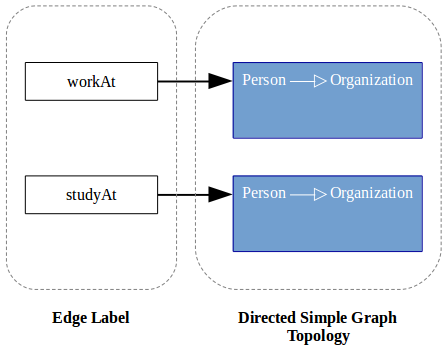
\includegraphics[width=5.5in]{Multi-graphTopology}
%\caption{Directed Multi-graph Topology}
%\label{fig_multiGraphTopology}
%\end{figure}

%In (\ref{fig_multiGraphTopology}), we are showing a block diagram for a logical representation of an example for a directed multi-graph. In the example, a directed multi-graph is stored between vertices of type \textit{"Person"} and \textit{"Organization"}, where the edges between the vertices are labeled as \textit{"workAt"} or \textit{"studyAt"}. We will store the directed multi-graph as a set of \textit{(key, value)} pairs, where the \textit{key} is the edge label and the \textit{value} is a graph topology data structure storing a directed simple graph for all edges labeled that have an edge label equal to \textit{key}.

We designed the graph topology data structures to facilitate the search, insert and retrieval of data in constant time by storing the data on multiple levels. Every data element we store in a graph topology data structure is consisted of three fields that represent a labeled relationship between two vertices. The three fields are \textbf{Source Vertex Id}, \textbf{Edge Label} and \textbf{Target Vertex Id}. An example for a three fields relationship is the relationship that exists in a social network graph between a post and its creator (e.g. \textit{post\_1 hasCreator person\_1}) with \textit{post\_1} represents the \textbf{Source Vertex Id}, \textit{hasCreator} represents the \textbf{Edge Label} and \textit{person\_1} represents the \textbf{Target Vertex Id}.

In the following subsections we are providing the technical details of our physical implementation for three graph topology data structures \textit{(Adjacency Matrix, Compressed Sparse Row and Adjacency List)}, as well as a parallel version of the \textit{Adjacency List} data structure that enables the ingestion of data from multiple parallel loaders. For every structure, we will present the building blocks we have utilized to build the data structure. Furthermore, we will explain the the mechanism and complexity for searching for an element inside the data structure.


%A graph is expressed mathematically as an ordered pair G = (E, V) with a set of edges E and a set of vertices V. In a directed graph, an edge (x, y) is a representation of the relationship between two vertices x and y, where x is the source vertex and y is the target vertex.



\begin{figure}
\centering
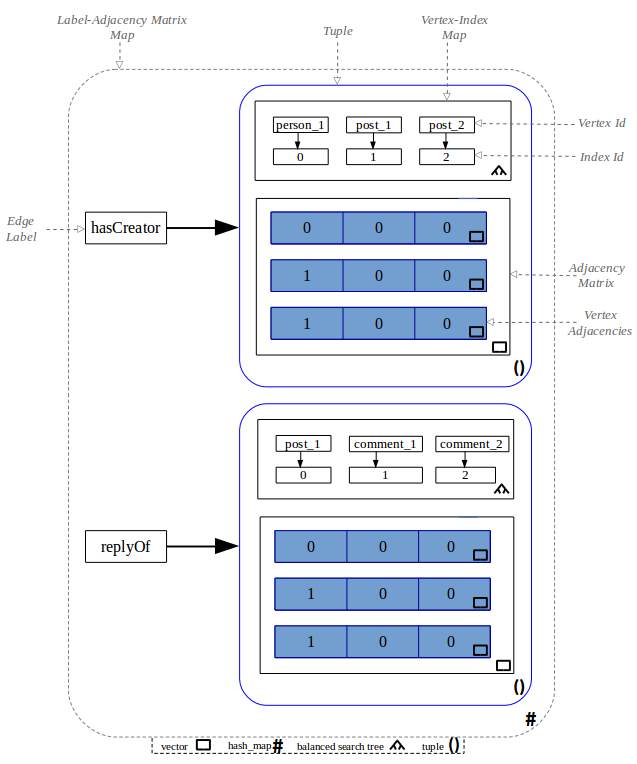
\includegraphics[height=7.8in]{adjacencyMatrix_physical}
\caption{Physical Representation of Labeled Adjacency Matrix}
\label{fig_adjacencyMatrix_physical}
\end{figure} 

\subsection{Adjacency Matrix}

In this subsection, we present our physical implementation of the labeled adjacency matrix data structure as one of the graph topology structures.

\begin{itemize}

\item{Structure:}

In (\ref{fig_adjacencyMatrix_physical}), we are presenting the underlying containers we utilized to implement the labeled adjacency matrix which which is basically defined as an adjacency matrix that is identified by the edge label of all possible edges between its vertices.

At the core of the structure, we store a two dimensional matrix serving as the \textit{Adjacency Matrix}. The size of the matrix is \textit{$n \times n$}. The row index id and column index id in the matrix are ranging from \textit{0} to \textit{n-1}. In addition, we store a \textit{Vertex-Index Map} that we use as a key/value store to associate each \textit{Vertex Id} with a corresponding \textit{Index Id} in the 2-d matrix. A \textit{Vertex Id} is always associated with one \textit{Index Id} which represents its row and column \textit{Index Id} in the 2-d matrix.

Each cell in the two dimensional matrix stores a boolean flag that indicates the existence of a relationship (i.e. flag = 1) between a source vertex which is associated with the row index of the cell, and a target vertex which is associated with the column index of the cell. A cell with "0" value means no relationship exists between the two vertices associated with the row and column index respectively.

%The \textit{Adjacency Matrix} space requirements is (\textit{O($n^2$)}) which for large graphs would be prohibitively expensive. For example, a graph of 10,000,000 vertex will require storage of size 11.6 petabyte.

In (\ref{fig_adjacencyMatrix_physical}), the \textit{Label-Adjacency Matrix Map} is a key/value store we use to associate every \textit{Edge Label} with a \textit{Tuple} that groups the \textit{Adjacency Matrix} and the \textit{Vertex-Index Map} in one container. Each \textit{Adjacency Matrix} will store the edge between the \textit{Source Vertex} and \textit{Target Vertex} which is labeled with the \textit{Edge Label} it's associated with.

\item{Insertion:}

To insert a new labeled relationship between two vertices into the structure, we first access the \textit{Label-Adjacency Matrix Map} using the \textit{Edge Label} as the access key. If no key exists with that \textit{Edge Label}, we insert a new key/value pair into the \textit{Label-Adjacency Matrix Map} with the key equal to the \textit{Edge Label} and the value is a \textit{Tuple} of empty \textit{Vertex-Index Map} and empty \textit{Adjacency Matrix}. Next, we retrieve the \textit{Index Ids} for the \textit{Source Vertex} and the \textit{Target Vertex} from the \textit{Vertex-Index Map}. In case any of the vertex ids of the source and target vertices not found in the \textit{Vertex-Index Map}, we insert a new key/value pair into the \textit{Vertex-Index Map} with the a key equal to the \textit{Source Vertex Id} and the value is \textit{m}, where \textit{m} is the number of pairs stored in the \textit{Vertex-Index Map} before the insertion. 

An insertion of new element(s) into the \textit{Vertex-Index Map} means that we must make a corresponding expansion in the \textit{Adjacency Matrix} to accommodate the relationship flags of the new elements(s). The \textit{Adjacency Matrix} is expanded by adding more columns and rows so that the final size of the matrix is equal to \textit{$m \times $m}, where \textit{m} is the number of pairs stored in the \textit{Vertex-Index Map}. The new cells added after expansion are all populated with a "0" value. 

Moreover, we use the \textit{Index Id} of the \textit{Source Vertex} as the row index and the \textit{Index Id} of the \textit{Target Vertex} as the column index in order to access a single cell at the \textit{Adjacency Matrix} and set the cell's flag to "1" to indicate an existence of a relationship between the \textit{Source Vertex} and the \textit{Target Vertex}.

\item{Searching:}

To search for a labeled relationship between two vertices in the structure, we first access the \textit{Label-Adjacency Matrix Map} using the \textit{Edge Label} as the access key. Next, we retrieve the \textit{Index Ids} for the \textit{Source Vertex} and the \textit{Target Vertex} from the \textit{Vertex-Index Map}. We use the retrieved \textit{Index Id} of the \textit{Source Vertex} as the row index and the \textit{Index Id} of the \textit{Target Vertex} as the column index in order to access a single cell at the \textit{Adjacency Matrix}.

If the cell holds a value of "1", it will mean that the relationship we are searching for does exist. A value of "0" would mean the opposite, that the relationship we are searching for does not exist.

The time complexity for the searching operation is the sum of complexity of three operations. First operation is accessing the \textit{Label-Adjacency Matrix Map} which has a complexity of \textit{O(1)}. Second operation is searching for the \textit{Index Id} for the \textit{Source Vertex} and the \textit{Target Vertex} from the \textit{Vertex-Index Map} which has a complexity of \textit{O(log(n) + log(n)) = O(2log(n))} where \textit{n} is the size of the \textit{Vertex-Index Map}. Third operation is accessing a cell in the \textit{Adjacency Matrix} which has a complexity of \textit{O(1)} for accessing the outer vector and \textit{O(1)} for accessing the inner vector which sums up to \textit{O(2)}.

By summing up the complexity of the three operations, the overall complexity of searching the structure is \textit{O(3 + 2log(n))}.

\item{Design Choices:}

We implemented the \textit{Label-Adjacency Matrix Map} as a static hash map to be the outer data container in the structure. The key of the hash map is the \textit{Edge Label}. As the number of \textit{Edge Labels} in a graph is not growing rapidly, the number of rehashing that is performed with the insertion of every new key will be limited. Meanwhile, the static hash map will give the best performance (\textit{O(1)}) for key look up operations on the \textit{Label-Adjacency Matrix Map}.

A graph can grow to include billions of vertices and hence the choice of a balanced search tree for implementing the \textit{Vertex-Index Map} as it guarantees a worst-case search or insert complexity for an element with \textit{O(log(size))}
(\cite{NSA}).

We chosen to implement the \textit{Adjacency Matrix} as a vector of vectors due to the the ability of the vector data structure to dynamically expand its capacity to store more elements in the run time. In addition, the vector data structure is storing its data contagiously in memory which enables the use of the principle of locality for efficient processing of the vector's data. Moreover, access operations on a vector is done in a constant time (\textit{O(1)}) which facilitates an efficient processing of the \textit{Adjacency Matrix's} data.

\end{itemize}

\subsection{Compressed Sparse Row (CSR)}

In this subsection, we present our physical implementation of the labeled compressed sparse row (CSR) data structure as one of the graph topology structures.



\begin{figure}[ht]
\centering
\hspace*{-0.4in}
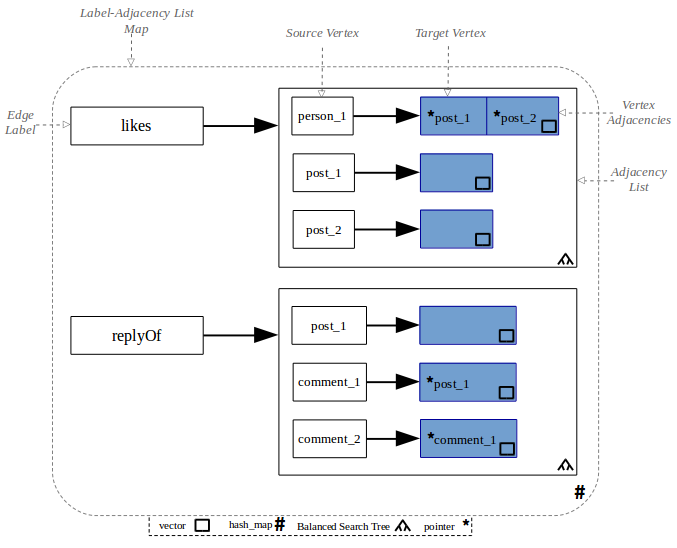
\includegraphics[width=6.8in]{adjacencyList_physical}
\caption{Physical Representation of Labeled Adjacency List}
\label{fig_adjacencyList_physical}
\end{figure}


\subsection{Adjacency List}
\label{adjList_physical}

In this subsection, we present our physical implementation of the labeled adjacency list data structure as one of the graph topology structures.

\begin{itemize}

\item{Structure:}

In (\ref{fig_adjacencyList_physical}), we are presenting the underlying containers we utilized to implement the labeled adjacency list which is basically defined as an adjacency list that is identified by the edge label of all possible edges between its vertices.

At the core of the structure, we store the \textit{Adjacency List} as a key/value store to associate each \textit{Source Vertex} with a corresponding sorted list of \textit{Target Vertices}. Each element of the list of \textit{Target Vertices}, is a direct pointer towards the key/value pair of the referenced \textit{Target Vertex} in the \textit{Adjacency List}.

In (\ref{fig_adjacencyList_physical}), the \textit{Label-Adjacency List Map} is a key/value store we use to associate every \textit{Edge Label} with an \textit{Adjacency List}. Each \textit{Adjacency List} will store the edge between the \textit{Source Vertex} and \textit{Target Vertex} which is labeled with the \textit{Edge Label} it's associated with.

\item{Insertion:}

To insert a new labeled relationship between two vertices into the structure, we first access the \textit{Label-Adjacency List Map} using the \textit{Edge Label} as the access key. If no key exists with that \textit{Edge Label}, we insert a new key/value pair into the \textit{Label-Adjacency List Map} with the key equal to the \textit{Edge Label} and the value is an empty \textit{Adjacency List}. Next, we access the \textit{Adjacency List} using the \textit{Source Vertex} as the key. Additionally, we retrieve a pointer to the key/value pair entry of the \textit{Target Vertex} from the \textit{Adjacency List}. In case we didn't find an entry with the given \textit{Source Vertex} or \textit{Target Vertex}, we insert a new key/value pair into the \textit{Adjacency List} with the key equal to the \textit{Vertex Id} and the value is an empty list. Lastly, we insert the pointer of the \textit{Target Vertex} into the list of \textit{Target Vertices} of the \textit{Source Vertex}, ensuring the insertion leaves the list sorted by the \textit{Vertex Id}.

\item{Searching:}

To search for a labeled relationship between two vertices in the structure, we first access the \textit{Label-Adjacency List Map} using the \textit{Edge Label} as the access key. Next, we access the \textit{Adjacency List} using the \textit{Source Vertex} as the key. Lastly, we search the list of \textit{Target Vertices} for a pointer to the given \textit{Target Vertex}.

The time complexity for the searching operation is the sum of complexity of three operations. First operation is accessing the \textit{Label-Adjacency List Map} which has a complexity of \textit{O(1)}. Second operation is is accessing the \textit{Adjacency List} which has a complexity of \textit{O(log(n))}, where \textit{n} is the number of key/value pairs stored in the \textit{Adjacency List}. Third operation is searching the list of \textit{Target Vertices} for a pointer to the given \textit{Target Vertex} which has a complexity of \textit{O(m)}, where \textit{m} is the size of the \textit{Target Vertices} list.

By summing up the complexity of the three operations, the overall complexity of searching the structure is \textit{O(1 + log(n) + m)}.

\item{Design Choices:}

Similar to the \textit{Label-Adjacency Matrix Map}, we implemented the \textit{Label-Adjacency List Map} as a static hash map to be the outer data container in the structure. The key of the hash map is the \textit{Edge Label}. The static hash map will give the best performance (\textit{O(1)}) for key look up operations on the \textit{Label-Adjacency List Map}.

A graph can grow to include billions of vertices and hence the choice of a balanced search tree for implementing the \textit{Adjacency List} as it guarantees a worst-case search or insert complexity for an element with \textit{O(log(size))}
(\cite{NSA}).

We chosen to implement the list of \textit{Target Vertices} as a vector due to the the ability of the vector data structure to dynamically expand its capacity to store more elements in the run time. In addition, the vector data structure is storing its data contagiously in memory which enables the use of the principle of locality for efficient processing of the vector's data. Moreover, access operations on a vector is done in a constant time (\textit{O(1)}) which facilitates an efficient processing of the list elements. Keeping the list of \textit{Target Vertices} sorted, makes the search for specific element in the list more efficient by utilizing a range of searching algorithms (e.g. binary search).

\end{itemize}


\subsection{Parallel Adjacency List}

In this subsection, we present our physical implementation of a parallel version of the adjacency list data structure. The parallel adjacency list differs from the adjacency list presented in (\ref{adjList_physical}) in that the parallel adjacency list enables the ingestion of data from multiple parallel loaders simultaneously.



\section{Graph Properties Structures}
\label{GraphPropertiesImp}


\subsection{Universal Table}


\subsection{Emerging Schema}


\subsection{Schema Hashed Map}


\subsection{Parallel Schema Hashed Map}


\section{Summary}
\label{summary}

}
{\chapter{Evaluation: Scalability and Data Loading}
\label{chap:Eval_4}

\section{Scalability}


\section{Bulk Data Loading}


\section{Parallel Data Loading}


\section{Summary}
}
{\chapter{Evaluation: Selection and Full Scan Queries}
\label{chap:Eval_5}


\section{Selection Queries}


\section{Full Scan Query}


\section{Summary}
}
{\chapter{Related Work}
\label{chap:RelatedWork}
}
.\ifgerman{\chapter{Zusammenfassung}}{\chapter{Conclusion and Future Work}
\label{chap:Conclusion}

}



%*********************************************************************%
% APPENDIX                                                            %
%*********************************************************************%

\appendix

%\include{chapters/appendixA}
%\include{chapters/appendixB}

%*********************************************************************%
% LITERATURE                                                          %
%*********************************************************************%

\cleardoublepage
\phantomsection
\addcontentsline{toc}{chapter}{\bibname} % 
\bibliographystyle{alpha} % plain gerplain abbrvnat unsrtnat alphag alpha
% in a thesis you have space... use full names
\bibliography{literature/IEEEfull,literature/MYfull,literature/literature}
% in a paper, space is limited. use abreviations
%\bibliography{../literature/IEEEabrv,../literature/MYabrv,../literature/literature}

%*********************************************************************%
% ERKLÄRUNG                                                           %
%*********************************************************************%

\ifnotdraft{
	\cleardoublepage
	\phantomsection
	\printindex
	\thispagestyle{empty}
\vspace*{38\baselineskip}



%%%%%%%%%%%%%%%%%%%%%%%%%%%%%%%%%%%%%%%%%%%%%%%%%%%%%%%%%%%%%%%%%%%%%%%%
%% Hinweis:
%%
%% Diese Erklärung wird von der Prüfungsordnung für Diplomarbeiten 
%% verlangt und ist zu unterschreiben. Für Studienarbeiten ist diese
%% Erklärung nicht zwingend notwendig, schadet aber auch nicht.
%%%%%%%%%%%%%%%%%%%%%%%%%%%%%%%%%%%%%%%%%%%%%%%%%%%%%%%%%%%%%%%%%%%%%%%%
\clearpage

}

\end{document}
